\documentclass[10pt,a4paper]{article}
\usepackage[utf8]{inputenc}
\usepackage{amsmath}
\usepackage{amsfonts}
\usepackage{amssymb}
\usepackage{tikz}
\usetikzlibrary{shapes, positioning, decorations.text}
\usepackage{wrapfig}

\begin{document}
\title{Trebuchet}
	\section{Optimum Release Angle}
		At what angle should a projectile be launched to achieve the greatest range?
		If the angle is too large the projectile will go very high but will not have much forward velocity.
		If the angle is too low the projectile will be moving forward very quickly but will not be in the air long enough to make it anywhere.
		What angle will balance these two scenarios and provide the optimum altitude with the best forward velocity?
		Do you have a guess? Think of throwing a ball. What angle do you use when you are trying to really get it to go far?
		Should we use that guess, or can we use our knowledge of math to \emph{prove} what will be the best angle?
		
		\begin{figure}
		\begin{tikzpicture}
			\draw[style=dashed] (0, 0) .. controls (2,3) and (6,3) .. (8, 0);
			\draw[->,ultra thick] (0,0)--(10,0) node[right]{$x$};
			\draw[->,ultra thick] (0,0)--(0,5) node[above]{$y$};
			\node[cross out, draw] at (8,0) {};
			\draw[->, thick] (0,0) -- (2,3) node[midway, above, sloped] (TextNode) {$V$};
			\draw (2,0) arc (0:56:2) node[pos=0.4, above] (TextNode) {\large{$\theta$}};
			\node at (8,-0.4) {$R$};
		\end{tikzpicture}
		\caption{What value of $\theta$ will produce the largest $R$?}
		\label{fig:launchAngle}
		\end{figure}
		
	\subsection{Breakup $V$ into its  X and Y Components}
		The first step is to break up our initial velocity vector $V$ into its two component vectors $V_x$ and $V_y$.
		This will tell us how fast our projectile is moving in these two directions.
		
		\begin{wrapfigure}{l}{0.44\textwidth}
		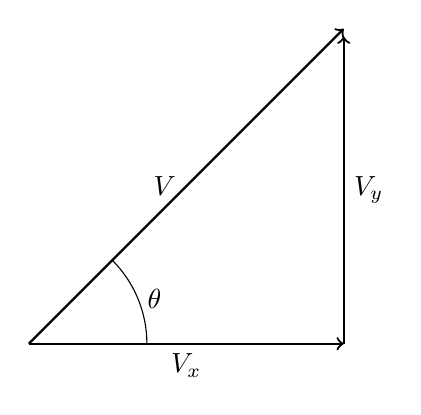
\begin{tikzpicture}
			\draw[->, thick] (0,0)--(4,0) node[below, midway] {$V_x$};
			\draw[->, thick] (4,0)--(4,3.9) node[right, midway] {$V_y$};
			\draw[->, thick] (0,0)--(4,4) node[left, midway] {$V$};
			\draw (1.5,0) arc (0:45:1.5) node[midway, right] {$\theta$};
		\end{tikzpicture}
		\caption{Component Vectors of $V$.}
		\label{fig:componentVectors}
		\end{wrapfigure}
		
		\noindent
		$V =$ launch velocity \\
		$\theta =$ launch angle \\
		$V_x =$ velocity in the $x$ direction \\
		$V_y =$ velocity in the $y$ direction \\
		
		How do we find the values of $V_x$ and $V_y$?
		Since we know that $V_x$ and $V_y$ form a right angle we can use the basic trig identities for $\sin, \cos, \tan$ to find the these values knowing only $V$ and $\theta$.
		Recall from trigonometry the mnemonic SOH-CAH-TOA.
		$V$ is our hypotenuse, H, and based on our $\theta$ location $V_y$ is the opposite, O, and $V_x$ is our adjacent, A.
		\clearpage
		With this information we can form the two equations:
		\[\sin\theta = \frac{V_y}{V} \quad, \quad \cos\theta = \frac{V_x}{V}\]
		Multiplying both sides of each equation by $V$ gives us the component vectors we want.
		\begin{equation}
			V_x = V \sin\theta \quad, \quad V_y = V \cos\theta
			\label{eq:componentVectors}
		\end{equation}
		
	\subsection{Distance Equation}
		Now that we know how fast the projectile is moving in each direction we can figure out far our projectile will travel.
		We know how fast the projectile is moving forward and if we knew how long it had to move forward we would know how far it went.
		The velocity in the y direction is what will determine how long our projectile will be in the air.		
		\begin{equation}
			S = X_i + V_i t + \frac{1}{2}at^2
			\label{eq:posEquation}
		\end{equation}
		where: \\
		$S =$ distance traveled \\
		$X_i =$ initial position \\
		$V_i = $ initial velocity \\
		$a =$ acceleration \\
		$t =$ time \\
		With this equation we can determine the position of our projectile in any one direction at any time.
		Since we need to know how long the projectile will be in the air we will work with $V_y$ first.
	\subsubsection{Flight Time}
		To determine how long the projectile will be in the air we can use just the $V_y$ component of our velocity vector and ignore $V_x$.
		We will assume that our projectile starts at $y=0$.
		It will be an exercise for the reader to determine if a higher starting height changes the optimum launch angle.
		We want to know the time, $t$, at which a projectile will return back to the ground after starting straight up at our initial velocity in y.
		Substituting in our known values we get the formula:
		\[\underbrace{0		\rule[-3pt]{0pt}{5pt}}_{\mbox{end pos}}
		  = \underbrace{0 		\rule[-3pt]{0pt}{5pt}}_{\mbox{initial pos}}
		  + \underbrace{V_yt	\rule[-3pt]{0pt}{5pt}}_{\mbox{$V\sin(\theta)t$}}
		  + \frac{1}{2}
		  \underbrace{-9.8		\rule[-3pt]{0pt}{5pt}}_{\mbox{gravity $m/s^2$}}
		  t^2  \]
		Please note that we are going to use metric units for gravity so all of our other units must be metric.
		Also, we have chosen to set "up" as positive y. 
		With this frame of reference gravity is pulling everything down, or accelerating objects down, so we need the negative sign. 
		This provides us with a quadratic equation which contains just one unknown value $t$.
		For equations with the form:
		\begin{equation}
			ax^2 + bx + c = 0
			\label{eq:quadratic}
		\end{equation}
		we can use the quadratic formula to solve for $x$.
		The quadratic formula is:
		\begin{equation}
			x = \frac{-b \pm \sqrt{b^2 - 4ac} }{2a}
			\label{eq:quadraticFormula}
		\end{equation}
		Rearranging our equation of motion to fit the form seen in equation \ref{eq:quadratic} we get:
		\[ \frac{1}{2}(-9.8)t^2 + V_yt + 0 = 0 \]
		where $a = \frac{1}{2}(-9.8) = -4.9, b = V_y,$ and $c = 0$.
		Substituting these values into the quadratic formula, eq. \ref{eq:quadraticFormula}:
		\[
			t = \frac{^- V_y \pm \sqrt{V_y^2 - 4 \times {^- 4.9} \times 0}}{2 \times \frac{1}{2} \times {^- 9.8}}
		\]
		Following through with the math:
		\[
			t = \frac{^- V_y \pm \sqrt{V_y^2}}{-9.8} = \frac{^- V_y \pm V_y}{-9.8}
		\]
		Now the $\pm$ means there are two possible solutions to our problem.
		If we look at the $+$ solution we see $-V_y + V_y$ in the numerator which equals 0.
		So we have a solution at $t=0$.
		What does this mean and does this make sense?
		Where is the projectile at $t=0$?
		$t_0$ is our start time and we said we are starting at $y=0$ so this makes sense and is a good check that our math is at least heading in the right direction.
		
		Taking a look at the minus solution we find:
		\[ t = \frac{^- V_y - V_y}{-9.8} = \frac{-2V_y}{-9.8}\]
		cancel out our negative signs and we arrive at our solution:
		\begin{equation}
			t = \frac{2V_y}{9.8}
			\label{eq:hangTime}
		\end{equation}
		This gives us our relation between our initial velocity in the y direction and how long the projectile will be in the air.
		The result is a positive number which makes sense since we are expecting the projectile to hit the ground some time after we have launched it and is proportional to the initial velocity, the faster we launch our object the longer it will stay in the air, and inversely proportional to the pull of gravity, if we were on a planet with stronger gravity it would stay in the air a shorter amount of time.
		
		Sanity check complete, now we will move on to the X direction and finally start calculating our range.
		
	\subsubsection{Range}
		Although you may already know that velocity $\times$ time $=$ distance, we will start with our equation of motion, eq \ref{eq:posEquation}, to ensure we have the correct answer and show how it all ties together. Substituting our $V_x$ values in for eq \ref{eq:posEquation} we get:
		\[ R = S = 0 + V_xt + \frac{1}{2}(0)t^2 \]
		Our initial position is again zero but this time our acceleration is also zero.
		An acceleration of zero in the X direction means nothing is slowing down the projectile in the forwards direction.
		Does this make sense?
		What about wind resistance?
		Doesn't that slow a projectile down?
		The answer is yes, and if we were going to account for wind resistance, also known as drag, it would be a negative acceleration placed in the last term.
		However, including drag makes the math much more difficult because it is not constant like gravity.
		Instead drag is a function of velocity which means it changes as the speed of our projectile changes.
		The faster our projectile is moving forward the more the wind pushes back.
		A typical drag formula is as follows:
		\[ F_d = \frac{1}{2}\rho v C_D A\]
		Where: \\
		$F_d =$ Drag force \\
		$\rho =$ Density of air \\
		$v =$ velocity, the part that will change with time \\
		$C_D =$ coefficient of drag, a number which can also change with velocity \\
		$A = $ cross sectional area \\
		Although accounting for wind resistance is not easy, we would also have to do it in the Y direction, it is not impossible.
		In fact with computers solving this problem is not necessary, we can instead choose small time steps where we assume the acceleration is constant and then after each time step, calculate the new velocity and then the new acceleration, and repeat.
		A task which can be done in Excel or with a simple WHILE/FOR loop in any programming language.
		
		Following through on our math for our range equation we find:
		\[ R = V_xt \]
		Our range is just our initial velocity $\times$ time, just as we expected.
		What is our time?
		That is eq \ref{eq:hangTime} from our Y calculations.
		Substituting in for $t$ we get:
		\[ R = V_x\left(\frac{2V_y}{9.8}\right) \]
		Now we can substitute in for $V_x$ and $V_y$ the values which relate them to our initial velocity and launch angle from eq \ref{eq:componentVectors}.
		\[ R = V\cos\theta \times V\sin\theta \times \frac{2}{9.8} \]
		Moving the constants out front we get:
		\begin{equation}
			R = \frac{2}{9.8} V^2 \cos(\theta) \sin(\theta)
			\label{eq:range}
		\end{equation}
		Now we need to find when this value is the maximum.
		
	\subsubsection{Maximum Range}
		
\end{document}